\documentclass[runningheads]{llncs}

\usepackage[hidelinks]{hyperref}
\usepackage{xcolor}
\usepackage{graphicx}
\usepackage{subcaption}
\usepackage{amsmath}
\usepackage{amssymb}
\usepackage{dsfont}
\usepackage{cite}
\usepackage{booktabs}
\usepackage{tabularx}
\usepackage{glossaries}
\usepackage{verbatim}
\usepackage[section]{placeins}

\makeatletter
\newenvironment{mycode}
 {\def\@xobeysp{\ }\verbatim\rightskip=0pt plus 6em\relax}
 {\endverbatim}
\makeatother
\newglossaryentry{Burden}{
    name=Burden,
    first={\emph{Burden}},
    description={A term we use for burden}
}
\newglossaryentry{statpar}{
    name=SP,
    first={\emph{statistical parity} (SP)},
    plural=statistical parities,
    description={}
}
% \newglossaryentry{statpar}{
%     name=statistical parity,
%     first={\emph{statistical parity}},
%     plural=statistical parities,
%     description={}
% }
\newglossaryentry{dempar}{
    name=demographic parity,
    first={\emph{demographic parity}},
    plural=demographic parities,
    description={}
}
\newglossaryentry{recourse}{
    name=recourse,
    first={\emph{recourse}},
    description={}
}
\newglossaryentry{sharma}{
    name=Sharma et al.~\cite{certifai},
    first={Sharma, Henderson, and Ghosh~\cite{certifai}},
    description={}
}
\newglossaryentry{legitimate}{
    name=legitimate,
    first={legitimate (non-sensitive and non-proxying)},
    description={}
}


\begin{document}

\title{Bursting the Burden Bubble?}
\subtitle{An Assessment of Sharma et al.'s Counterfactual-Based Fairness Metric}

\author{
Yochem van Rosmalen
\and
Florian van der Steen
\and
Sebastiaan Jans
\and
Daan van der Weijden
}

\authorrunning{Y. van Rosmalen et al.}

\institute{
Utrecht University, Heidelberglaan 8, 3584 CS Utrecht, The Netherlands\\
\email{\{y.m.vanrosmalen,f.a.vandersteen,s.j.j.jans,d.j.vanderweijden\}@students.uu.nl}}

\maketitle

\begin{abstract}
Machine learning has seen an increase in negative publicity in recent years,
due to biased, unfair, and uninterpretable models. There is a rising
interest in making machine learning models more fair for unprivileged
communities, such as women or people of color. Metrics are needed to
evaluate the fairness of a model. A novel metric for evaluating fairness
between groups is Burden, which uses counterfactuals to approximate the
average distance of negatively classified individuals in a group to the
decision boundary of the model. The goal of this study is to compare Burden
to statistical parity, a well-known fairness metric, and discover Burden's
advantages and disadvantages. We do this by calculating the Burden and
statistical parity of a sensitive attribute in three datasets: two
synthetic datasets are created to display differences between the two
metrics, and one real-world dataset is used. We show that Burden can be
more nuanced than statistical parity, but also that the metrics can
disagree on which group is treated unfairly. We therefore conclude that
Burden is a valuable metric to add to the existing group of fairness
metrics, but should not be used on its own.
\keywords{Fairness metrics \and Burden \and Statistical parity \and Decision
    boundary \and Sensitive attributes \and Unprivileged groups \and
    Classification}
\end{abstract}

\section{Introduction}

The use of algorithms in automated decision making has increased over the past
years, due to the increased accuracy in which they can predict or classify
desired outcomes. However, many of these algorithms are black boxes, whose
decision process is not transparent to humans. This is undesirable since it
could lead to the unfair treatment of certain groups, without being able to
provide an explanation \cite{angwin2016machine}. This has led to an increased
demand of fair and explainable models, with many new frameworks for providing
explanations being proposed
\cite{lundberg2017shap,ribeiro2016lime,ribeiro2018anchors}, as well as new
metrics to measure the fairness of a model
\cite{kamiran2009demographicparity,hardt2016equalisedodds,woodworth2017learning}.

Metrics for fair machine learning measure how well a particular model is
towards different groups within a dataset. Although the definition and
practical implementation of fairness varies between different metrics, their
overarching goal is to provide insight into the level of fairness between
different groups regarding sensitive attributes (e.g. age, gender,
socioeconomic status).

One of the new frameworks is CERTIFAI \cite{certifai}, a framework that tests
the robustness of a model, as well as providing explanations and a metric to
measure fairness. It does so by generating counterfactuals for each datapoint
in the dataset. This counterfactual is a synthetic datapoint, generated to have
the other possible outcome, while being as close as possible to the original
datapoint. The counterfactual provides insight as to what features should
change to have the model classify the datapoint differently. Not only does this
provide an explanation for why a certain classification was made, this also
allows us to measure the -- possibly unfair -- difference in treatment for
certain groups (e.g. male and female). By calculating the average distance for
a group between original datapoints in the negative outcome class (e.g. loan
application denied) and their generated counterfactuals (e.g. loan application
approved), the \gls{Burden} of a group can be calculated. The \gls{Burden} of
groups can be compared, in order to address which groups have a higher
\gls{Burden} and thus have more `difficulty' converting from the negative to
the positive predicted outcome class.

\gls{sharma} claim that this metric for fairness, which they call \gls{Burden},
is a more nuanced version of other fairness metrics, like \gls{statpar}, which
is a formal non-discrimination criterion used to measure fairness
\cite{kamiran2009demographicparity}. It is calculated by measuring the ratio of
the probability of receiving a positive outcome from a model between groups
(See Sec. \ref{sec:sp}). However, this claim is not validated in their study.
In this study, the claim is tested, by comparing the \gls{Burden} metric to
\gls{statpar}. We focus on \gls{statpar} because it, and \gls{Burden} likewise,
does not take the actual ground truth target value into account but rather the
model's prediction. This is clear in the formula for \gls{statpar}
(Eq.~\ref{eq:sp}). This matter is more in-depth explained in Sec.
\ref{sec:relatedwork}.

In this study, we investigate situations where both metrics give different
results to see if \gls{Burden} can provide more nuance and if it is a good
fairness metric in practice. This is tested on two synthetic datasets with
hypothetical data and a real-world loan application dataset \cite{dataset}. All
three datasets have a \emph{binary} outcome class: a favorable outcome and an
unfavorable outcome. This means that the models used are also binary
classification models.

\section{Related Work}\label{sec:relatedwork}

In this section, the fairness metrics \gls{statpar} (Sec.~\ref{sec:sp}) and
\gls{Burden} (Sec.~\ref{sec:burden}) are explained more in-depth to get a
better theoretical understanding of how and why they work as fairness metric.

\subsection{Statistical Parity}\label{sec:sp}
There are many metrics to measure how fair a model is, and there is no
agreement on a best method, or even on the definition of fairness itself
\cite{chouldechova2018frontiers}. However, one of the most common and easy to
implement fairness metrics is that of \gls{statpar}, or \gls{dempar}
\cite{kamiran2009demographicparity}. In order to calculate \gls{statpar}, we
have to calculate the acceptance rate (AR) for a specific group of $S$ e.g. if
$S$ is a binary value the groups could be 0 and 1, which can be seen in Eq
\ref{eq:ar}.
\begin{equation}\label{eq:ar}
 AR_{S=s} = P(\hat{Y}=1|S=s)
\end{equation}
This means that the acceptance rate of the group where $S=s$ is defined as the
probability ($P$) of the model predicting a positive outcome
($\hat{Y}=1$)\footnote{The actual ground truth outcome, or target value, of a
supervised dataset is denoted as $Y$, while the model's predicted outcome is
denoted as $\hat{Y}$.}, given that $S=s$. To calculate the \gls{statpar}
between two groups of a binary feature $S$, we look at the ratio of the
acceptance rate of both groups, as seen in Eq \ref{eq:sp}.
\begin{equation}\label{eq:sp}
    SP_{S} = \frac{P(\hat{Y}=1|S=0)}{P(\hat{Y}=1|S=1)}
\end{equation}
If the same percentage of individuals receives a positive score for each group,
and thus the outcome of the ratio is 1, the two groups both have the same
probability of receiving a positive outcome prediction from the model. This is
seen as fair: if $S$ is a sensitive attribute, e.g. age, there should be no
difference in receiving a positive prediction. Perfect \gls{statpar} is almost
never possible in practice, so often a maximum difference of 20\% is used, to
follow the 80\% rule for disparate impact \cite{feldman2015certifying}.

\subsection{Burden}\label{sec:burden}

In 2020, a new method of measuring fairness is proposed in the CERTIFAI
framework \cite{certifai}, where counterfactuals are used to measure different
treatment of groups. The use of counterfactuals for explanatory purposes is not
new \cite{mothilal2020DICE}, as is using counterfactuals to check if features
are proxies for known sensitive features
\cite{kusner2017counterfactual-fairness}.

A counterfactual, in this context, is a datapoint calculated to be as similar
to an original datapoint as possible, while receiving a different
classification. A counterfactual datapoint can provide an individual with
\gls{recourse}: the counterfactual datapoint can show the individual which
changes to the input features are necessary in order to change the
qualification to the desired output class.

\Gls{sharma} propose a genetic heuristic search for generating a counterfactual
$c$ for a datapoint $x$. The process is shown visually in
Fig.~\ref{fig:cf-generation}. Starting from a randomly generated population of
size $N$, the counterfactuals, $\mathbf{c}$, that are classified to be in the
opposing class are selected. These are then mutated with probability $P_m$,
which involves arbitrarily changing some feature values. Subsequently,
crossover is applied with probability $P_c$, which involves randomly
interchanging some feature values between individuals. Then, a top-$k$
selection procedure is applied where only the most fit counterfactuals are
selected. The fitness function $d(x,c)$ is a distance function calculated over
the datapoint and the counterfactual. The population is then filled back up to
$N$ by randomly generating new counterfactual points. This process is repeated
for a predetermined maximum of generations. Finally, the fittest counterfactual
$\mathbf{c^*}$ is selected.

With these fittest counterfactuals, the \gls{Burden} of a group can be
calculated. The \gls{Burden} of a group with value $s$ for feature $S$ is
defined as the mean of the distances between the datapoints in $S=s$ that had
an unfavorable decision and their counterfactuals,
\begin{equation}
    \text{Burden}_{S=s} = \mathbb{E}_{S=s}[d(\mathbf{x}, \mathbf{c^*})],
\end{equation}
where the distance function $d(\mathbf{x}, \mathbf{c^*})$ can be chosen.
Examples include the Manhattan ($L_1$) distance and the Euclidean ($L_2$)
distance.

\begin{figure}
    \centering
    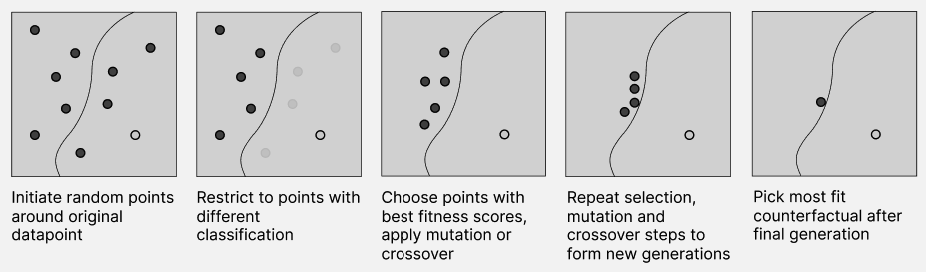
\includegraphics[width=\textwidth]{img/counterfactual_generation.png}
    \caption{Visual representation of the counterfactual generation process of
    CERTIFAI. Adopted from \cite{certifai}.}
    \label{fig:cf-generation}
\end{figure}

For a binary sensitive attribute, the average distances can be divided by each
other to give a ratio. If the ratio is larger than 1, the group in the
numerator has a greater \gls{Burden}, and if the ratio is smaller than 1, the
group in the denominator has a greater \gls{Burden}. An important difference
between the two fairness metrics is that with the acceptance rate,
\emph{higher} is better, but with Burden, \emph{lower} is better.

Remark that it is hard to verify that any difference in \gls{Burden} between
groups is not a measurement error, e.g. because of badly generated
counterfactuals, due to the dimensionality of the data or complexity of the
model. In this paper, however, we assume that any found difference in Burden is
a true difference and it correctly implies that members in the unprivileged
group have greater difficulty changing their outcome.



\section{Methods}\label{sec:methods}
In this section, we describe the methodology of this study. The methodology is
broken down in four parts: the creation of the two synthetic datasets, the
description of the `Default of Credit Card Clients' dataset, the classifier
models and lastly CERTIFAI's counterfactuals and Burden. The Python code
(Jupyter Notebook), saved models and generated data is available on
GitHub\footnote{\url{https://github.com/yochem/bursting-the-burden-bubble}}.

\subsection{Synthetic Datasets}\label{sec:syndata}

We created two datasets to demonstrate two types of disagreements between
\gls{Burden} and \gls{statpar} that are theoretically possible. One synthetic
dataset, $D_A$, shows that \gls{Burden} disagrees with \gls{statpar} about if
\textit{there is} unfairness, and the other dataset, $D_B$, shows that
\gls{Burden} disagrees with \gls{statpar} about \emph{which group} is treated
unfairly. Both synthetic datasets consist of 80 datapoints.

Each datapoint in the two datasets consists of three features and a label. The
\gls{legitimate}\footnote{A proxying feature can reveal sensitive information.
E.g. someones address, although not a sensitive feature, can reveal someones
socioeconomic status because of their neighborhood.} features $X_1$ and $X_2$,
the sensitive attribute $S$ (0 is unprivileged, 1 is privileged), and the
target label $Y$ (0 is unfavorable, 1 is favorable). This means that datapoint
$i$ is given by $ D^{(i)} = (x_1, x_2, s, y)$. The \gls{legitimate} features
$X_1$ and $X_2$ are both sampled from normal distributions ($X \sim
\mathcal{N}(\mu, \sigma^2)$) with different means $\mu$. All samples have a
standard deviation $\sigma^2$ of 1. The sensitive attribute $S$ is selected
(not sampled from a random distribution), as is the target label $Y$. The true
underlying function between the legitimate features and the outcome can be
derived from Table~\ref{tab:syndata}.

\subsubsection{Dataset on Presence of Unfairness $D_A$}

\gls{Burden} takes the average distance of a group to their counterfactuals
into account, while \gls{statpar} does not. Therefore, the synthetic data needs
to satisfy two properties: Firstly, it needs to satisfy \gls{statpar}, so for
each group, the same number of datapoints needs to be predicted positive.
Secondly, the average distance of the negatively predicted datapoints to their
counterfactuals needs to differ between the two groups to show how \gls{Burden}
can find this unfairness.

As described in Section~\ref{sec:syndata}, the \gls{legitimate} features $X_1$
and $X_2$ are sampled from a normal distribution and $S$ and $Y$ are selected.
Sensitive attribute groups $S=0$ and $S=1$ both have a probability of 0.5 on
the favorable outcome, which is considered fair according to the \gls{statpar}
metric, i.e. $P(\hat{Y}=1|S=0) = P(\hat{Y}=1|S=1) = 0.5$. The same is the case
for target label $Y$. The distribution of dataset $D_A$ is shown in
Table~\ref{tab:syndata}. The datapoints of synthetic dataset $D_A$ are plotted
in Fig.~\ref{fig:syndatafavor}, along with their counterfactuals.

\subsubsection{Dataset on Direction of Unfairness $D_B$}

This dataset should let \gls{Burden} and \gls{statpar} disagree on which group
is treated unfairly. This means that \gls{statpar} has to label one group of
the sensitive attribute as unprivileged, and \gls{Burden} has to label the
other group as unprivileged. \Gls{statpar} labels a group as unprivileged if
the group has less positively predicted outcomes as the other group
($P(\hat{Y}=1|S=0) \neq P(\hat{Y}=1|S=1)$). When we have a perfect classifier
(accuracy of 1), $\hat{Y} = Y$. Using the definition of \gls{statpar}, an
unprivileged group can be formed by having relatively fewer datapoints where
$\hat{Y}=1$. For \gls{Burden} to disagree with \gls{statpar}, the other
$S$-group (i.e. the group that \gls{statpar} sees as privileged) needs to have
a greater distance to their counterfactuals at the decision boundary, as
illustrated in Fig. \ref{fig:cf-generation}.

To create a synthetic dataset with these properties, the distributions of
proposed dataset $D_B$ is shown in Table~\ref{tab:syndata}. Note that
$P(\hat{Y}=1|S=0)\approx0.57$ and $P(\hat{Y}=1|S=1)\approx0.67$, and therefore
has an imbalance in the positive outcome rates between the two groups, if the
classifier has perfect accuracy. The average distance to the counterfactuals
and thus the \gls{Burden} however is higher for group $S=1$. The datapoints of
synthetic dataset $D_B$ are shown in Fig.~\ref{fig:syndataunfavor}, along with
their counterfactuals.

\begin{table}
    \centering
    \caption{The distribution of values per feature for both datasets $D_A$ and
    $D_B$. The count is the number of datapoints sampled from the normal
    distributions for $X_1$, and $X_2$, with shown mean $\mu$ for their normal
    distribution $\mathcal{N}(\mu, 1)$.}
    \label{tab:syndata}
    \begin{tabularx}{.7\textwidth}{@{\extracolsep{\fill}}cccccccccc}
        \toprule
        \multicolumn{5}{c}{Dataset $D_A$} & \multicolumn{5}{c}{Dataset $D_B$}\\
        \cmidrule(lr){1-5}\cmidrule(lr){6-10}
        $\mu_{X_1}$ & $\mu_{X_2}$ & $S$ & $Y$ & count & $\mu_{X_1}$ & $\mu_{X_2}$ & $S$ & $Y$ & count\\
        \midrule
        1 & 9 & 0 & 0 & 20 & \hspace{0.2cm} 1 & 9 & 1 & 0 & 15\\
        3.5 & 5 & 1 & 0 & 20 &\hspace{0.2cm} 3.5 & 5 & 0 & 0 & 15\\
        9 & 1 & 0 & 1 & 20 &\hspace{0.2cm}  9 & 1 & 1 & 1 & 30\\
        9 & 1 & 1 & 1 & 20 & \hspace{0.2cm} 9 & 1 & 0 & 1 & 20\\
        \bottomrule
    \end{tabularx}
\end{table}

\subsection{Default of Credit Card Clients Dataset}\label{sec:taiwan}

To explore the claim of \gls{Burden} being more nuanced, the metric is also
compared to \gls{statpar} on real-world data. This is done on a subset of the
Default of Credit Card Clients dataset, also known as the Taiwan loan dataset,
from \cite{dataset} (from now on called Taiwan dataset). This is a dataset of
credit card users, which records whether the individual defaults on a loan.
Since defaulting on a loan is a negative outcome, the favorable label in this
dataset is 0: `did not default'. The unfavorable label is 1: `default'. The
sensitive attributes are gender, education, marriage,, and age \cite{eusex}. In
our experiments we treat gender as the sensitive attribute. Monthly payments
were tracked for the other features, such as history of past payment, amount of
bill statement, amount of previous payment,, and amount of given credit. More
information on these features can be found in \cite{dataset}. Datapoints with
incorrect values were removed. The dataset contains 30,000 instances. The
computational cost for generating counterfactuals is large because the genetic
algorithm iteratively goes over large population sizes for many generations.
Therefore, this study is limited to a random sample of 1000 instances from the
Taiwan dataset.


\subsection{Classifier}\label{sec:model}

A binary classification model (classifier) is needed for calculating
\gls{Burden}, and \gls{statpar}. The choice of classifier is not very important
for this study, because the counterfactuals can be learned independent of the
model's internals. On all three datasets, a Logistic Regression model
\cite{cox1958regression} was trained. This model was chosen because it is
complex enough to learn a perfect decision boundary for the synthetic datasets,
and it is traditionally used for this task \cite{crook2007recent}.

The classifiers were trained on the datasets without their sensitive features.
No hyper-parameter optimization was performed, and the datasets were not
partitioned into separate tests for training, and evaluation. This was done to
remove unnecessary complexity: our interest lies in evaluating fairness, not
model performance. The Logistic Regression model was implemented in PyTorch for
reasons concerning compatibility with the CERTIFAI framework. It used the
binary cross-entropy loss function \cite{cox1958regression}, and the stochastic
gradient descent optimizer \cite{robbins1951stochastic}. The learning rate was
0.001, and was trained using 2000 iterations. The number of input dimensions
for each classifier was the number of \gls{legitimate} features, i.e. $X_1$ and
$X_2$ for the synthetic datasets, and 19 features for the Taiwan dataset
relating to past payments, bill statements, and credit features.

\subsection{CERTIFAI's Burden}\label{sec:certifai}

Using the \texttt{CERTIFAI.fit()} method, counterfactuals were generated given
the model. The hyperparameters were the following: 10 generations of
populations with size 60,000, of which maximal 10,000 retain after selection,
of which maximal 5,000 retain for the next generation, and unconstrained
generating of counterfactual features. The probabilities for crossover and
mutation were adopted from \cite{certifai}. For calculating the Burden,
CERTIFAI's \texttt{check\_fairness} method was used with as argument a mapping
containing 1) the sensitive attribute and its value (e.g. \texttt{s: 0}), and
2) that it should be calculated over the unfavorable class (i.e.
\texttt{favorable: 0}).

\section{Results}\label{sec:results}

\begin{figure}
    \centering
    \begin{subfigure}{0.49\textwidth}
        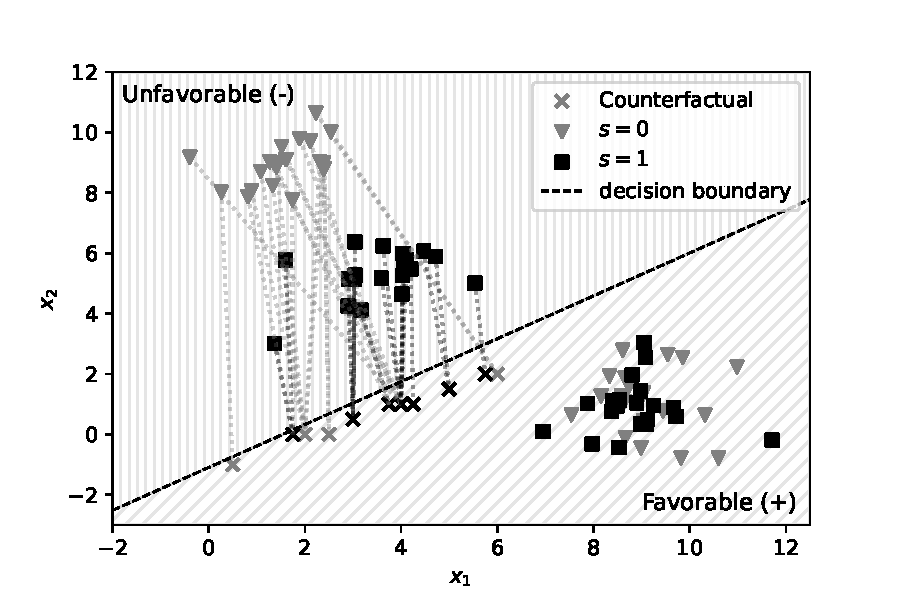
\includegraphics[width=\textwidth]{img/syndata-A-bw}
        \caption{$D_A$, where \gls{Burden} and \gls{statpar} disagree on the
        presence of unfairness.}
        \label{fig:syndatafavor}
    \end{subfigure}
    \begin{subfigure}{0.49\textwidth}
        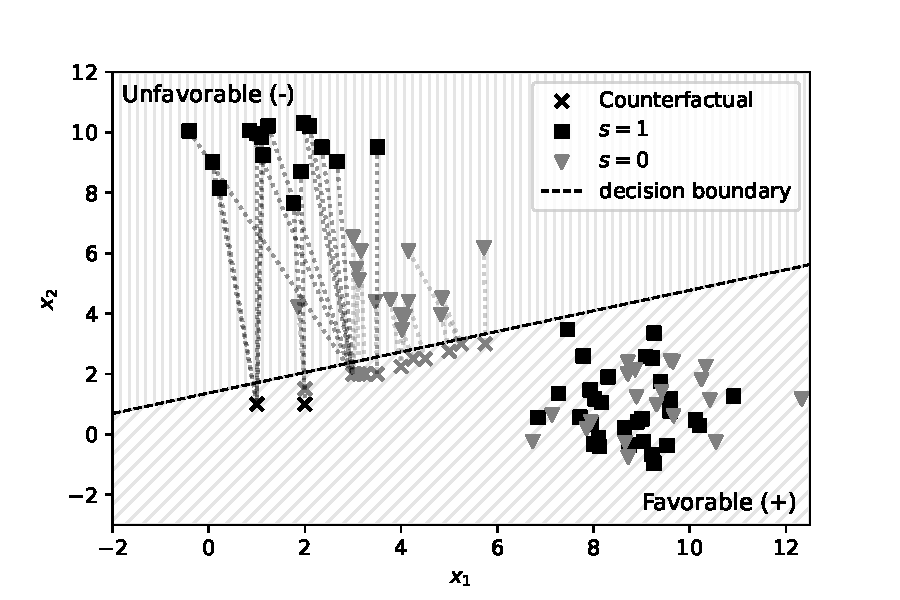
\includegraphics[width=\textwidth]{img/syndata-B-bw}
        \caption{$D_B$, where \gls{Burden} and \gls{statpar} disagree on the
        direction of unfairness.}
        \label{fig:syndataunfavor}
    \end{subfigure}
    \caption{The synthetic datapoints ($\blacktriangledown,\blacksquare$) for
    datasets $D_A$ and $D_B$. The counterfactuals (\texttimes) for datapoints
    from the unfavorable outcome class are also included and are connected
    using a dotted line. The decision boundary (\texttt{---}) of the classifier
    is also shown.}
    \label{fig:syndataplot}
\end{figure}

In the first two experiments, logistic regression models were trained on $D_A$
and $D_B$ respectively and both got an accuracy of 1.00. In Fig.
\ref{fig:syndataplot}, this is shown by the decision boundaries laying
perfectly between both groups. After the models were trained, the
counterfactuals for the unfavorable class were generated by CERTIFAI, also
shown in Fig. \ref{fig:syndataplot}. After this, the \gls{statpar} and
\gls{Burden} were calculated. The results of the metrics on both experiments
are listed in Table \ref{table:results}.

For the experiment on $D_A$ we see that the \gls{statpar} is met, thus having a
ratio of 1 between groups. The Burden of group $S=0$ is higher (Burden of 11.6)
than of group $S=1$ (Burden of 4.65). This difference in Burden can also be
eyeballed using Fig.~\ref{fig:syndatafavor}, where the $S=0$ group is further
away from their counterfactuals than the $S=1$ group.

For the experiment on $D_B$ we see that the ratio in \gls{statpar} is 0.857.
The Burden of the two groups are 3.31 and 11.0 for $S=0$ and $S=1$,
respectively. The datapoints are plotted in Fig.~\ref{fig:syndataunfavor}.

The results of the last experiment, on the Taiwan dataset, are also listed in
Table \ref{table:results}. The model trained on this dataset achieved an
accuracy of 0.78. The results are the following: \Gls{statpar} is nearly met,
with a value of 1.02 (0.967 over 0.948). \Gls{Burden} however shows that
females have almost 1.5x higher Burden than males, respectively 1.38 and 0.940.

\begin{table}
    % als je deze tabel aanpast, ctrl+f de waardes ff om te kijken of ze ergens
    % genoemd worden. Vooral in discussie!
    \centering
    \caption{\Gls{statpar} and \gls{Burden} for the three datasets. The
    acceptance rate and \gls{Burden} are given per group ($S=0$ and $S=1$ for
    the synthetic datasets correspond to gender=female and gender=male
    respectively for the Taiwan dataset), as well as the \gls{Burden} ratio and
    statistical parity (SP) between the two groups, in bold.}
    \label{table:results}
    \begin{tabularx}{.8\textwidth}{l@{\extracolsep{\fill}}cccccc}
    \toprule
    & \multicolumn{2}{c}{Acceptance Rate} & SP & \multicolumn{3}{c}{Burden}\\
    \cmidrule(lr){2-3}\cmidrule(lr){4-4}\cmidrule(lr){5-7}
    % & \multicolumn{2}{c}{$S$} & ratio  & \multicolumn{2}{c}{$S$} & ratio\\
    % \cmidrule(lr){2-3}\cmidrule(lr){4-4}\cmidrule(lr){5-6}\cmidrule(lr){7-7}
    Dataset & $S=0$ & $S=1$ & 0/1 & $S=0$ & $S=1$ & 0/1\\
    \midrule
    Taiwan & 0.967 & 0.948 & \textbf{1.02} & 1.38 & 0.940 & \textbf{1.47}\\
    $D_A$  & 0.500 & 0.500 & \textbf{1.00} & 11.6 & 4.65 & \textbf{2.49}\\
    $D_B$  & 0.571 & 0.667 & \textbf{0.857} & 3.31 & 11.0 & \textbf{0.302}\\
    \bottomrule
    \end{tabularx}
\end{table}



\section{Discussion}\label{sec:discussion}

In this section, the results are discussed as well as the limitations of this
study and directions for future work.

\subsection{Discussion on Experimental Results}

In the first experiment with dataset $D_A$, the results show that even though
\gls{statpar} was met (ratio of 1.00), Burden shows that the model is unfair
towards group $S=0$, since their Burden is higher. This means that Burden can
show unfairness between groups when \gls{statpar} can not. This is a positive
result for the claim of \gls{sharma} that \gls{Burden} provides more nuance
than \gls{statpar} in this situation. The distance to the counterfactuals near
the decision boundary is important here to actually find the unfairness.

In the second experiment on dataset $D_B$, the \gls{statpar} shows unfairness
towards group $S=0$ since \gls{statpar} is less than 1. Burden however tells us
that group $S=1$ is being treated unfairly, because the Burden of this group
(11.0) is higher than the Burden of the other group (3.31). This means that
\gls{statpar} and Burden can disagree on which group is treated unfairly.

As a third experiment, on real-world Taiwan data, the results show the same
effect as the first experiment. Although the difference is smaller than with
$D_A$, the results show that with \gls{statpar} the model is more fair than
with Burden. Burden can thus add more nuance than \gls{statpar}.

\subsection{Limitations and Future Work}

Future work could find real-world examples of the synthetic dataset $D_B$, and
if the disagreement between \gls{Burden} and \gls{statpar} found in our
synthetic experiment occurs in other situations.

Furthermore, it is important to note that the computational complexity of the
\gls{Burden} metric is extremely high in comparison to a metric like
\gls{statpar}. While \gls{statpar} is a simple calculation of a ratio between
two percentages, the calculation of a single counterfactual for the
\gls{Burden} metric can take minutes. For large datasets it might thus be
necessary to compute this metric for a representative sample of the dataset.

To conclude the discussion, which of \gls{statpar} and \gls{Burden} is the
better metric, and for which use-case, is a matter of subjective debate. It is
in general a matter of subjective debate how fairness should be expressed in a
number, or in fact even whether that is really possible or desirable at all
\cite{corbett2018measure}. Different stakeholders value different aspects of
fairness differently. In fact, popular fairness metrics such as \gls{statpar}
and equalized odds \cite{hardt2016equality} are mutually exclusive under
reasonable assumptions \cite{chouldechova2017fair}, which shows the extent of
differences between metrics.

\section{Conclusion}\label{sec:conclusion}

In this study we assessed the fairness metric introduced in \gls{sharma}, using
three experiments. The first experiment, using synthetic dataset $D_A$, shows
that \gls{Burden} can pick up unfairness when \gls{statpar} can not. The second
experiment, using synthetic dataset $D_B$, shows that \gls{Burden} and
\gls{statpar} can even disagree on which group is treated unfairly. The last
experiment, using the Taiwan dataset, shows that \gls{Burden} is more nuanced
than \gls{statpar} on a real-world dataset. The three experiments show that
\gls{Burden} can provide more information than \gls{statpar}, but this
information may not be in line with \gls{statpar}.

We therefore conclude that \gls{Burden} should not replace \gls{statpar} or any
other fairness metric, because they measure  different aspects of fairness. The
advantage of using \gls{Burden} as fairness metric is taking distance into
account, which can provide more information about underlying unfairness between
groups. The biggest disadvantage of \gls{Burden} is the computational
complexity. Therefore, considering its additional costly information about
fairness, on large datasets, Burden can be applied on a random sample that
reflects the global statistics of the original dataset.

\subsubsection*{Acknowledgments.}

We thank dr. Dong Nguyen, Yupei Du, and dr. Heysem Kaya for their great help.

\bibliographystyle{splncs04}
\bibliography{references}

\end{document}
